\documentclass{book}
\input{latexmacro}
\usepackage{graphicx}

\begin{document}
\setcounter{chapter}{3}

% special version of Chapter 4 for Luis to edit to create Java version
% 6/9/2012  6/26/2012  6/27/2012  7/2/2012
% definitions added just for this version
\newtheorem{example}{Example}[chapter]
\def\ttf{\texttt{TTF}}
\def\Clock{\texttt{Clock}}
\def\Entity{\textttf{Entity}}
\def\D{\mathrm{d}}
% end special definitions

\chapter{Simulation Programming with VBASim}
\label{ch:vbasim}
\index{VBASim}

This chapter shows how simulations of some of the examples in
Chap.~\ref{ch:examples} can be programmed in VBASim. The goals of
the chapter are to introduce VBASim, and to hint at the experiment
design and analysis issues that will be covered in later
chapters. A complete listing of the VBASim source code can be found in
Appendix~\ref{app:VBASim}. \index{VBASim}

\section{VBASim Overview}
\label{sec:vbasim.overview}

VBASim is a collection of VBA Subs, Functions and Class Modules that
aid in developing discrete-event simulations. They are entirely open
source and can be modified to suit the user. The random-number and
random-variate generation routines are VBA translations of the
corresponding routines in simlib (Law 2007) which is written in
\texttt{C}.\index{Law, A. M.}\index{simlib} VBASim is designed to be
easy to understand and use, but not necessarily efficient. 


Here is a brief description of the Subs and Functions in VBASim:
\begin{description}

\item[\texttt{Sub VBASimInit:}] Initializes VBASim for use, typically
called before the start of each replication.

\item[\texttt{Sub Schedule:}] Schedules future events.

\item[\texttt{Sub SchedulePlus:}] Schedules future events and allows
an object to be stored with the event.

\item[\texttt{Sub Report:}] Writes a result to a specific row and
column of an Excel worksheet.

\item[\texttt{Sub ClearStats:}] Clears certain statistics being recorded
by VBASim.

\item[\texttt{Sub InitializeRNSeed:}] Initializes the
random-number generator; typically called only once in a simulation.

\item[\texttt{Function Expon:}] Generates exponentially
distributed random variates. 

\item[\texttt{Function Uniform:}] Generates uniformly 
distributed random variates. 

\item[\texttt{Function Random\_integer:}] Generates a random
integer. 

\item[\texttt{Function Erlang:}] Generates Erlang
distributed random variates. 

\item[\texttt{Function Normal:}] Generates normally
distributed random variates. 

\item[\texttt{Function Lognormal:}] Generates lognormally
distributed random variates. 

\item[\texttt{Function Triangular:}] Generates triangularly
distributed random variates. 

\end{description}


The random-variate generation functions take two types of
arguments: parameters, and a random-number stream; the random-number
stream is always the last argument. For instance
\begin{center}
\texttt{X = Uniform(10, 45, 2)}
\end{center}
generates random-variates that are uniformly distributed between $10$
and $45$, using stream $2$. 

As you already know, the pseudorandom numbers we use to generate
random variates in simulations are essentially a long list.
Random-number streams are just different starting places in this
list, spaced far apart. The generator in VBASim (which is a
translation of the generator in Law 2007) has $100$ streams. Calling
\texttt{Sub InitializeRNSeed} sets the initial position of each
stream. Then each subsequent call to a variate-generation routine
using stream \# advances stream \# to the next pseudorandom number.
The need for streams is discussed in Chap.~\ref{ch:output}, but it
is important to know that any stream is as good as any other stream
in a well-tested generator. \index{random-number stream}


Here is a brief description of the Class Modules (objects) in VBASim:
\begin{description}

\item[\texttt{Entity:}] Object used to model transient items that
flow through the system. 

\item[\texttt{FIFOQueue:}] Object to hold entities in
first-in-first-out order.

\item[\texttt{Resource:}] Object used to model a scarce quantity.

\item[\texttt{EventNotice:}] Object used to represent a future event.

\item[\texttt{EventCalendar:}] Data structure holding event notices in
chronological order.

\item[\texttt{CTStat:}] Object used to record continuous-time
statistics.

\item[\texttt{DTStat:}] Object used to record discrete-time
statistics.

\end{description}




\section{Simulating the $M(t)/M/\infty$ Queue}
\label{sec:sim.mminf}

\def\Calendar{\texttt{Calendar}}
\def\Schedule{\texttt{Schedule}}
\def\Remove{\texttt{Remove}}
\def\EventType{\texttt{EventType}}
\def\EventTime{\texttt{EventTime}}
\def\EventNotice{\texttt{EventNotice}}
\def\CTStat{\texttt{CTStat}}
\def\TheCTStats{\texttt{TheCTStats}}
\def\tN{\texttt{N}}
\def\MaxQueue{\texttt{MaxQueue}}


Here we consider the parking lot example of Sect.~\ref{sec:mminf},
a queueing system with time-varying car arrival rate, exponentially
distributed parking time and an infinite number of parking spaces.
The simulation program consists of some global declarations
(Fig.~\ref{fig:parking.declare}), a main program and some event
routines (Fig.~\ref{fig:parking.main}), an initialization sub
(Fig.~\ref{fig:parking.init}), a function to generate car arrivals
(Fig.~\ref{fig:parking.nspp}), and the support functionality
provided by VBASim.  Two important aspects of VBASim are illustrated
by this model: event scheduling and collecting time-averaged
statistics. 

%And we describe how the simulation can be used to decide how many
%spaces to have in the parking lot. 

The key state variable that we need to track is the number of cars in
the lot. There are two essential events that affect the state, the
arrival of a car and the departure of a car, and a third event we
will use to stop the simulation at a specific point in time. The
tricky part is that there can be an unlimited number of pending
``departure'' events; in fact, there are as many pending departure
events as there are cars in the lot. Therefore, having a unique
variable to represent the scheduled time of each pending event, as
was used for the \ttf\ example in Chap.~\ref{ch:quick}, will not
work. 

\begin{sloppypar}

To handle event scheduling, VBASim has an event calendar data
structure called \Calendar, a sub called \Schedule\ for putting
events on the \Calendar, and a method called \Remove\ for extracting
the next event from the calendar. An event in VBASim is a VBA
object of class \EventNotice\ which has (at least) two properties:
\EventType\ and \EventTime. The statement 
\begin{center}
\Schedule\texttt{(Name, Increment)} 
\end{center}
creates an \texttt{EventNotice}, assigns the character
string \texttt{Name} to the \EventType\ property, assigns the value
\texttt{Clock + Increment} to the \EventTime\ property, and schedules
the \texttt{EventNotice} on the \Calendar\ in the correct
chronological order. The method \texttt{Calendar.Remove} extracts the
chronologically next \texttt{EventNotice} from the \Calendar, 
making its \EventType\ and \EventTime\ properties available to
advance time and execute the proper event.

The simulation main program \texttt{Sub MtMInf} in
Fig.~\ref{fig:parking.main} illustrates how the event-related
features of VBASim work.  The following four statements, or ones very
similar, will appear in all simlations using VBASim:
\begin{verbatim}
Dim NextEvent As EventNotice

Set NextEvent = Calendar.Remove
Clock = NextEvent.EventTime
Select Case NextEvent.EventType
\end{verbatim}

Since our simulation will repeatedly remove the next
\texttt{EventNotice} from \Calendar, we need an object of this class
to which to assign it; the statement \texttt{Dim NextEvent As
EventNotice} provides this. The statement \texttt{Set NextEvent =
Calendar.Remove} illustrates how the \Remove\ method extracts the
next event, after which we advance the simulation \Clock\ to time
\texttt{NextEvent.EventTime} and execute the event indicated by
\texttt{NextEvent.EventType}.  

VBASim's \Schedule\ sub places events on the \Calendar; for instance,
the statement 
\begin{center}
\texttt{Call Schedule("EndSimulation", 24)} 
\end{center}
creates an
\texttt{EventNotice} of type EndSimulation to occur $24$ hours from
the time currenly on \Clock\ (which is $0$ at the beginning of the
simulation). Notice that VBASim requires the user to decide on the
base time unit in the simulation and to use it consistently
throughout. In this simulation the base time unit is hours.



\begin{figure}[tbp]
\begin{minipage}[t]{6in}\small
\begin{verbatim}
' Example illustrating use of VBASim for simulation of M(t)/M/infinity Queue
' parking lot example.
' In this version parking time averages 2 hours;
' the arrival rate varies around 100 per hour;
' the lot starts empty, and we look at a 24-hour period.
' 
' See VBASim module for generic declarations
' See Class Modules for the supporting VBASim classes
' Parameters we may want to change
Dim MeanParkingTime As Double

' Simulation variables and statistics
Private N As Integer                'Number in queue
Dim QueueLength As New CTStat       'Use to keep statistics on N
Private MaxQueue As Integer         'Largest observed value of N
\end{verbatim}
\end{minipage}
\caption{Declarations for the parking lot simulation.}
\label{fig:parking.declare}
\end{figure}


\begin{figure}[tbp]
\begin{minipage}[t]{6in}\small
\begin{verbatim}
Private Sub MtMInf()
' Initialize
    Dim Reps As Integer
    Dim NextEvent As EventNotice
    Call MyInit ' special one-time initializations    
    For Reps = 1 To 1000
    ' Initializations for each replication
        N = 0
        MaxQueue = 0
        Call VBASimInit 'initialize VBASim for each replication
        Call Schedule("Arrival", NSPP(1))
        Call Schedule("EndSimulation", 24)
        Do
            Set NextEvent = Calendar.Remove
            Clock = NextEvent.EventTime
            Select Case NextEvent.EventType
            Case "Arrival"
                Call Arrival
            Case "Departure"
                Call Departure
            End Select
        Loop Until NextEvent.EventType = "EndSimulation"
' Write output report for each replication
        Call Report(QueueLength.Mean, "MtMInf", Reps + 1, 1)
        Call Report(MaxQueue, "MtMInf", Reps + 1, 2)
    Next Reps
    End ' ends execution, closes files, etc.
End Sub

Private Sub Arrival()
' Arrival event
' Schedule next arrival
    Call Schedule("Arrival", NSPP(1))
' Update number in queue and max
    N = N + 1
    QueueLength.Record (N)
    If N > MaxQueue Then
        MaxQueue = N
    End If
' Schedule departure
    Call Schedule("Departure", Expon(MeanParkingTime, 2))
End Sub

Private Sub Departure()
' End of service event
' Update number in queue
    N = N - 1
    QueueLength.Record (N)
End Sub
\end{verbatim}
\end{minipage}
\caption{Main program and event routines for the parking lot
simulation.}
\label{fig:parking.main}
\end{figure}



The key state variable in this simulation is \tN, the current number
of cars in the parking lot, and we want statistics on it.  VBASim
contains a \CTStat\ class that can be used to record time-averaged
statistics. Here is how it works: First, we declare a new \CTStat\
using the statment 
\begin{center}
\texttt{Dim QueueLength As New CTStat} 
\end{center}
as shown in the global declarations (Fig.~\ref{fig:parking.declare}).
Second, the \CTStat\ can (and usually should) be added to a special
collection called \TheCTStats, as shown in
Fig.~\ref{fig:parking.init}. VBASim reinitializes any \CTStat\ in
\TheCTStats\ collection whenever \texttt{Call VBASimInit} is executed,
which is typically at the beginning of each replication.  Next,
whenever the value of the variable of interest changes, the
\texttt{Record} method of the \CTStat\ is employed to record the
change (which means it is called just after the change occurs); in
this simulation the statement is \texttt{QueueLength.Record (N)}, as
shown in Fig.~\ref{fig:parking.main}. Finally, the time-averaged value
of the \CTStat\ can be computed using the \texttt{Mean} method of the
\CTStat, as in \texttt{QueueLength.Mean}.  

\end{sloppypar}

Notice that VBASim also has a \texttt{Report} sub that writes a value or
character string to a given row and column of an Excel worksheet. The
syntax is
\begin{center}
\texttt{Call Report(value or string, worksheet, row, column)}
\end{center}
See Figs.~\ref{fig:parking.main} and~\ref{fig:parking.init}.


\begin{figure}[tbp]
\begin{verbatim}
Private Sub MyInit()

' Initialize the simulation
    Call InitializeRNSeed
    MeanParkingTime = 2
    TheCTStats.Add QueueLength

' Write headings for the output reports

    Call Report("Average Number In Queue", "MtMInf", 1, 1)
    Call Report("Maximum Number in Queue", "MtMInf", 1, 2)

End Sub
\end{verbatim}
\caption{Initializing the parking lot simulation.}
\label{fig:parking.init}
\end{figure}



Recall that the arrival rate (in cars per hour) to the parking lot
was modeled by the function $\lambda(t) = 1000 + 100\sin(\pi t/12)$.
To make the simulation execute more quickly for the purpose of
this introduction, we change that rate to $\lambda(t) = 100 + 10\sin(\pi
t/12)$, so that the arrival rate varies between $90$ and $110$
cars per hour, depending on the hour of the day $t$.

The \texttt{Function NSPP} shown in Fig.~\ref{fig:parking.nspp}
generates interarrival times (time gaps between arrivals) from a
nonstationary Poisson process \index{nonstationary Poisson process}
with this arrival rate. The formal definition of a nonstationary
Poisson process is a topic of Chap.~\ref{ch:input}.  However, we
provide an intuitive justification for the working of
\texttt{Function NSPP} here:

A stationary Poisson process has times between arrivals that are
exponentially distributed with a fixed rate $\lambda$ (or
equivalently a constant mean time between arrivals $1/\lambda$).  The
inverse cdf method for generating exponentially distributed random
variates was described in Chap.~\ref{sec:random.variates}.  \index{inverse
cdf} The maximum arrival rate for $\lambda(t)$ is $110$ cars per
hour, so \texttt{Function NSPP} generates possible arrivals using a
stationary arrival process with rate $\lambda = 110$. To achieve the
time-varying arrival rate, it only accepts a \emph{possible} arrival at time
$t$ as an \emph{actual} arrival with probability $\lambda(t)/\lambda$.  Thus,
a possible arrival that is to occur at a time when $\lambda(t) = 110$
will always be an actual arrival, while a possible arrival that is to
occur when $\lambda(t) = 90$ will only have a $90/110$ probability of
being an actual arrival. That this method, which is called
``thinning,'' generates a nonstationary Poisson process with the
desired rate is discussed in Chap.~\ref{ch:input}.\index{thinning}


\begin{figure}[tbp]
\begin{verbatim}
Private Function NSPP(Stream As Integer) As Double
' This function implements thinning to generate interarrival times
' from the nonstationary Poisson arrival process representing
' car arrivals. Time units are minutes.

Dim PossibleArrival As Double

PossibleArrival = Clock + Expon(1 / 110, Stream)

Do Until Uniform(0, 1, Stream) < _
        (100 + 10 * VBA.Sin(3.141593 * PossibleArrival / 12)) / 110
    PossibleArrival = PossibleArrival + Expon(1 / 110, Stream)
Loop

NSPP = PossibleArrival - Clock

End Function
\end{verbatim}
\caption{Function to generate interarrival times to the parking lot.}
\label{fig:parking.nspp}
\end{figure}


Fig.~\ref{fig:mminfaverage} shows a histogram of the $1000$ daily
averages of the number of cars in the parking lot obtained by running
the simulation for $1000$ replications; the overall average of these
averages is $184.2 \pm 0.3$ cars, where the ``$\pm 0.3$'' part comes
from a $95$\% confidence interval on the mean (confidence intervals
are a subject of Chap.~\ref{ch:output}). Thus, the simulation
provides a pretty precise estimate of the time-average mean number of
cars that would be found in the (conceptually) infinite-size garage
during a day.


\begin{figure}[tb]
\centerline{\includegraphics[width=4in]{mminfaverage.eps}}
\caption{Histogram of the daily average number of cars.}
\label{fig:mminfaverage}
\end{figure}


The histogram shows that the average number of cars in the garage can
vary substantially from day to day, so we certainly would not want to
build a garage with a capactity of, say, $185$ cars. Further,
averaging over the day masks the largest number of cars in the garage
during the day, and that number is more useful for selecting a finite
capacity for the garage.  

VBASim provides no special support for the maximum statistic, but
since we have access to everything in a VBASim simulation we can
easily record whatever we want. Here we define a variable \MaxQueue\
which is initialized to $0$ at the beginning of each
replication, and is increased to the current value of \tN\ whenever
\tN\ exceeds the previous value of \MaxQueue. See in particular
\texttt{Sub Arrival} in Fig.~\ref{fig:parking.main}. 

Suppose that we want the parking lot to be of adequate size $99$\% of
the time. Since we record the maximum size on $1000$ replications, we
could use the $990$th value (sorted from smallest to largest) as the
size of the garage, which turned out to be 263 cars in this
simulation.  Figure~\ref{fig:mminfmax} shows the empirical cumulative
distribution (ecdf) \index{ecdf} of the $1000$ maximums recorded by
the simulation. The ecdf treats each observed value as equally likely
(and therefore as having probability $1/1000$), and plots the sorted
maximum values on the horizontal axis and the cumulative probability
of each observation on the vertical axis. The plot shows how the
cumulative probability of $0.99$ maps to the value of $263$ cars,
which might be a very reasonable capacity for the garage. Putting a
confidence interval on this value is quite different than putting one
on the mean, and will be discussed in Chap.~\ref{ch:output}.
Without a confidence interval (or some measure of error) we cannot be
sure if $1000$ replications is really enough to estimate the $99$th
percentile of the maximum. 


\begin{figure}[tb]
\centerline{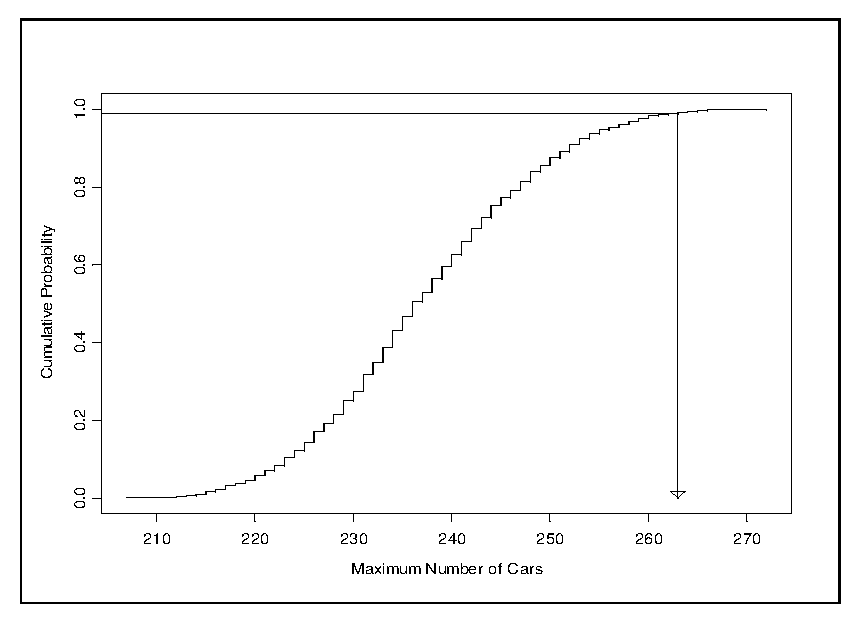
\includegraphics[width=4in]{mminfmax.eps}}
\caption{Empirical cdf of the daily maximum number of cars in the
parking lot.}
\label{fig:mminfmax}
\end{figure}


\subsection{Issues and Extensions}
\label{sec:sim.mminf.issues}

\begin{enumerate}

\item The $M(t)/M/\infty$ simulation presented here simulates $24$
hours of parking lot operation, and treats each $24$-hour period
as as independent replication starting with an empty garage. This only
makes sense if the garage is emptied each day, for instance if the
mall closes at night. Is the assumed arrival rate $\lambda(t)$
appropriate for a mall that closes at night?

\item Suppose that the parking lot serves a facililty that is
actually in operation $24$ hours a day, seven days per week (that is,
all the time). How should the simulation be initialized, and how long
should the run length be in this case?

\item How could the simulation be initialized so that there are $100$
cars in the parking lot at time $0$? 

\item When this example was introduced in Sect.~\ref{sec:mminf}, it
was suggested that we size the garage based on the (Poisson)
distribution of the number of cars in the garage at the point in time
when the mean number in the garage was maximum. Is that what we did,
empirically, here? If not, how is the quantity we estimated by
simulation related to the suggestion in Sect.~\ref{sec:mminf} (for
instance, will the simulation tend to suggest a bigger or smaller
garage than the analytical solution in Sect.~\ref{sec:mminf})?

\item One reason that this
simulation executes quite slowly when $\lambda(t) = 1000 +
100\sin(\pi t/12)$ is that the thinning method we used is very
inefficient (lots of possible arrivals are rejected). Speculate about
ways to make it faster.

\item For stochastic processes experts: Another reason that the
simulation is slow when $\lambda(t) = 1000 + 100\sin(\pi t/12)$ is
that there can be $1000$ or more pending departure events on
\Calendar\ at any time, which means that scheduling a new event in
chronological order involves a slow search. However, it is possible
to exploit the memoryless property of the exponential distribution of
parking time to create an equivalent simulation that has only two
pending events (the next car arrival and next car departure) at any
point in time. Describe how to do this.

\end{enumerate}


\section{Simulating the $M/G/1$ Queue}
\label{sec:sim.mg1}

Here we consider the hospital example of Sect.~\ref{sec:mg1}, a
queueing system with Poisson arrival process, some (as yet
unspecified) service-time distribution, and a single server (either a
receptionist or an electronic kiosk); in other words, an $M/G/1$
queue.\index{$M/G/1$ queue} Patient waiting time is the key system
performance measure, and the long-run average waiting time in
particular.

Recall that Lindley's Equation~(\ref{eq:lindley}) provides a shortcut
way to simulate  successive customer waiting times:\index{Lindley's Equation}
\begin{eqnarray*}
Y_0 &=& 0 \qquad X_0 = 0 \\
Y_i &=& \max\{0, Y_{i-1} + X_{i-1} - A_i\},\ i=1,2,\ldots
\end{eqnarray*}
where $Y_i$ is the $i$th customer's waiting time, $X_i$ is that
customer's service time, and $A_i$ is the interarrival time between
customers $i-1$ and $i$. Lindley's equation avoids the need for an
event-based simulation, but is limited in what it produces (how would
you track the time-average number of customers in the queue?). In
this section we will describe both recursion-based and event-based
simulations of this queue, starting with the recursion.

\subsection{Lindley Simulation of the $M/G/1$ Queue}
\label{sec:sim.mg1.lindley}

To be specific, suppose that the mean time between arrivals is $1$
minute, with the distribution being exponential, and the mean time to use
the kiosk is $0.8$ minutes ($48$ seconds), with the distribution
being an Erlang-$3$.\index{Erlang distribution} An Erlang-$p$ is the
sum of $p$ i.i.d.\ exponentially distributed random variables, so an
Erlang-$3$ with mean $0.8$ is the sum of $3$ exponentially
distributed random variables each with mean $0.8/3$.

In Sect.~\ref{sec:mg1} we noted that the waiting-time
random variables $Y_1, Y_2, \ldots$ converge in distribution to a
random-variable $Y$, and it is $\mu = \E(Y)$ that we will use to
summarize the performance of the queueing system. We also noted that
$\bar{Y}(m) = m^{-1}\sum_{i=1}^m Y_i$ converges with probability $1$
to $\mu$ as the number of customers simulated $m$ goes to infinity.

All of this suggests that we make a very long simulation run (large
$m$) and estimate $\mu$ by the average of the observed waiting times
$Y_1, Y_2, \ldots, Y_m$. But this is not what we will do, and here is
why: Any $m$ we pick is not $\infty$, so the waiting times early in
the run---which will tend to be smaller than $\mu$ because
the queue starts empty---will likely pull $\bar{Y}(m)$ down. To
reduce this effect, we will let the simulation generate waiting times
for a while (say $d$ of them) before starting to actually include
them in our average. We will still make $m$ large, but our average
will only include the last $m-d$ waiting times. That is, we will use as
our estimator the truncated average \index{truncated average}
\begin{equation}
\label{eq:truncated.average}
\bar{Y}(m,d) = \frac{1}{m-d}\sum_{i=d+1}^m Y_i .
\end{equation}
In addition, we will not make a single run of $m$ customers, but
instead will make
$n$ replications. This yields $n$ i.i.d.\ averages $\bar{Y}_1(m,d),
\bar{Y}_2(m,d),
\ldots, \bar{Y}_{n}(m,d)$ to which we can apply standard statistical
analysis. This avoids the need to directly estimate the asymptotic
variance $\gamma^2$, a topic we defer to later chapters.



\begin{figure}[tbp]
\begin{verbatim}
Private Sub Lindley()

Dim Rep As Integer
Dim m As Long, i As Long
Dim d As Integer
Dim Y As Double, X As Double, A As Double
Dim SumY As Double

Call Report("Average Wait", "Lindley", 1, 1)
Call InitializeRNSeed
m = 55000
d = 5000
    
For Rep = 1 To 10
    Y = 0
    SumY = 0
    For i = 1 To d
        A = Expon(1, 1)
        X = Erlang(3, 0.8, 2)
        Y = WorksheetFunction.Max(0, Y + X - A)
    Next i
    For i = d + 1 To m
        A = Expon(1, 1)
        X = Erlang(3, 0.8, 2)
        Y = WorksheetFunction.Max(0, Y + X - A)
        SumY = SumY + Y
    Next i
    Call Report(SumY / CDbl(m - d), "Lindley", Rep + 1, 1)
Next Rep
End

End Sub
\end{verbatim}
\caption{Simulation of the $M/G/1$ queue using Lindley's equation.}
\label{fig:hospital.lindley}
\end{figure}

Figure~\ref{fig:hospital.lindley} shows a VBASim simulation of the
$M/G/1$ queue using Lindley's equation. In this simulation
$m=55{,}000$ customers, we discard the first $d=5000$ of them, and
make $n=10$ replications. 
The ten replication averages are individually written to an Excel
worksheet called ``Lindley'' and are displayed in
Table~\ref{tab:lindley.results}. 

Notice that the average waiting time
is a bit over $2$ minutes, and that VBA, like all programming
languages, displays a very large number of output digits. How many
are really meaningful? A confidence interval is one way to provide an
answer.

Since the across-replication averages are i.i.d., and since each
across-replication average is itself the within-replication average
of a large number of individual waiting times ($50{,}000$ to be
exact), the assumption of independent, normally distributed output
data is reasonable. This justifies a $t$-distribution confidence
interval on $\mu$.\index{$t$ distribution} The key ingredient is
$t_{1 - \alpha/2, n-1}$, the $1-\alpha/2$ quantile of the $t$
distribution with $n-1$ degrees of freedom. If we want a $95$\%
confidence interval, then $1 - \alpha/2 = 0.975$, and our degrees of
freedom are $10 - 1 = 9$. Since $t_{0.975, 9} = 2.26$, we get
$2.148759113 \pm (2.26) (0.066748617)/\sqrt{10}$ or $2.148759113 \pm
0.047703552$.  This implies that we can claim with high confidence
that $\mu$ is around $2.1$ minutes, or we could
give a little more complete information as $2.14 \pm 0.05$ minutes.  Any
additional digits are statistically meaningless.

Is an average of $2$ minutes too long to wait? To actually answer
that question would require some estimate of the corresponding wait
to see the receptionist, either from observational data or a
simulation of the current system. Statistical comparison of
alternatives is a topic of Chap.~\ref{ch:DandA}.


\begin{table}[tbp]
\caption{Ten replications of the $M/G/1$ queue using Lindley's
equation.}
\label{tab:lindley.results}
\begin{center}
\begin{tabular}{cc}\hline
replication&$\bar{Y}(55000, 5000)$ \\\hline
1	&2.191902442\\
2	&2.291913404\\
3	&2.147858324\\
4	&2.114346960\\
5	&2.031447995\\
6	&2.110924602\\
7	&2.132711743\\
8	&2.180662859\\
9	&2.139610760\\
10	&2.146212039 \\\hline
average	&2.148759113\\
std dev&0.066748617 \\\hline
\end{tabular}
\end{center}
\end{table}



\subsection{Event-based Simulation of the $M/G/1$ Queue}
\label{sec:sim.mg1.event}

\def\FIFOQueue{\texttt{FIFOQueue}}
\def\Entity{\texttt{Entity}}
\def\Resource{\texttt{Resource}}
\def\DTStat{\texttt{DTStat}}
\def\CreateTime{\texttt{CreateTime}}
\def\ClearStats{\texttt{ClearStats}}


\begin{figure}[tbp]
\begin{verbatim}
' Example illustrating use of VBASim for
' simulation of M/G/1 Queue.

' See VBASim module for generic declarations
' See Class Modules for the supporting VBASim classes

' Parameters we may want to change
Private MeanTBA As Double        ' mean time between arrivals
Private MeanST As Double         ' mean service time
Private Phases As Integer        ' number of phases in service distribution
Private RunLength As Double      ' run length
Private WarmUp As Double         ' "warm-up" time

' Global objects needed for simulation
' These will usually be queues and statistics

Dim Queue As New FIFOQueue          'customer queue
Dim Wait As New DTStat              'discrete-time statistics on customer waiting
Dim Server As New Resource          'server resource
\end{verbatim}
\caption{Declarations for the hospital simulation.}
\label{fig:hospital.declare}
\end{figure}

The simulation program consists of some global declarations
(Fig.~\ref{fig:hospital.declare}), a main program
(Fig.~\ref{fig:hospital.main}), some event routines
(Fig.~\ref{fig:hospital.events}), an initialization sub
(Fig.~\ref{fig:hospital.init}), and the support functionality
provided by VBASim.  Four VBASim class objects and one sub are illustrated by
this model: \Entity, \FIFOQueue, \Resource\, \DTStat\ and \ClearStats. At a high
level, here is what they do:
\begin{itemize}

\item \Entity\ objects are used to model transient items, such as
transactions or customers that pass through the system. They can have
attributes (VBA properties) that they carry with them;  by default
they have an attribute called \CreateTime\ which is set to the value 
of \Clock\ when an \Entity\ object is created. In this
simulation the \Entity\ objects represent patients or visitors.

\item \FIFOQueue\ is a VBA Collection, much like \Calendar, that is
used for holding \Entity\ objects in first-in-first-out order; it
also records time-average number in the queue statistics. In this
simulation the queue represents the patients using or waiting for
the kiosk. 

\item \Resource\ objects represent scarce quantities like workers,
machines and computers that are needed (typically) to serve or
process an \Entity\ in some way; they also record the average number
of busy resource units. In this simulation the \Resource\ object
represents the kiosk.

\item \DTStat\ is an object for recording discrete-time statistics;
it is the companion to \CTStat\ for continuous-time statistics. In
this simulation a \DTStat\ is used to record total waiting-time statistics,
where we will define ``total waiting time'' to be the time from
patient arrival until they are finished with the kiosk. Notice that
this is (intentionally) different from the definition in
Sect.~\ref{sec:sim.mg1.lindley}, where the wait only included the
time to reach the front of the line.

\def\TheDTStats{\texttt{TheDTStats}}

\item \ClearStats\ is a sub that reintializes all statistical
variables found in two collections, \TheCTStats\ and \TheDTStats.
\FIFOQueue\ and \Resource\ objects each create a \CTStat\ which is
automatically added to \TheCTStats. When the programmer creates a
custom \CTStat\ or \DTStat\ then they must add it to the
appropriate collection.

\end{itemize}

\begin{figure}[tbp]
\begin{verbatim}
Private Sub MG1()
' Initialize

    Dim Reps As Integer
    Dim NextEvent As EventNotice

    Call MyInit ' special initializations for this simulation
    
    For Reps = 1 To 10
    
        Call VBASimInit 'initialize VBASim for each replication
    
        Call Schedule("Arrival", Expon(MeanTBA, 1))
        Call Schedule("EndSimulation", RunLength)
        Call Schedule("ClearIt", WarmUp)
    
        Do
            Set NextEvent = Calendar.Remove
            Clock = NextEvent.EventTime
            Select Case NextEvent.EventType
            Case "Arrival"
                Call Arrival
            Case "EndOfService"
                Call EndOfService
            Case "ClearIt"
                Call ClearStats
            End Select
        Loop Until NextEvent.EventType = "EndSimulation"

' Write output report for each replication

        Call Report(Wait.Mean, "MG1", Reps + 1, 1)
        Call Report(Queue.Mean, "MG1", Reps + 1, 2)
        Call Report(Queue.NumQueue, "MG1", Reps + 1, 3)
        Call Report(Server.Mean, "MG1", Reps + 1, 4)
    
    Next Reps
    
    End ' ends execution, closes files, etc.
    
End Sub
\end{verbatim}
\caption{Main program for the hospital simulation.}
\label{fig:hospital.main}
\end{figure}

Figure~\ref{fig:hospital.declare} shows the declarations of the
\FIFOQueue, \DTStat\ and \Resource\ objects, specifically:
\begin{verbatim}
Dim Queue As New FIFOQueue          
Dim Wait As New DTStat              
Dim Server As New Resource          
\end{verbatim}
These are declared globally because there is only one of each and
they will be referenced from many places in the simulation code.

\begin{sloppypar}

This contrasts with the \Entity\ objects that will be created and
discarded as needed to represent patients coming and going. For
instance, consider these four statements in \texttt{Sub Arrival}:
\begin{verbatim}
Dim Customer As New Entity
Queue.Add Customer
Set Customer = Nothing
\end{verbatim}
The keyword \texttt{New} in the \texttt{Dim} statement causes a new
instance of the \Entity\ class to be created. We can access its
attributes using the \texttt{.} extension, as in
\texttt{Customer.CreateTime}. The \texttt{Add} method of the
\FIFOQueue\ object \texttt{Queue} places \Entity\ objects into the
queue in order of arrival. Finally, the \texttt{Set Customer =
Nothing} statement frees the name \texttt{Customer} to be used again
for a new \Entity. This statement is not absolutely necessary unless
we execute the statement \texttt{Dim Customer As New Entity} a second
time within \texttt{Sub Arrival} because the name \texttt{Customer}
will automatically be released when we exit the \texttt{Sub}.
However, we think it is good programming practice to release the
object name when it is no longer needed so there is no confusion.
Notice that the \Entity\ object is not lost because it is stored in
\texttt{Queue}.

Moving into the \texttt{Sub EndOfService} event routine, the following four
statements remove the first customer from the queue, use its
\CreateTime\ attribute to compute the total waiting time, record
this value using the \DTStat\ object \texttt{Wait}, and finally
release the name \texttt{DepartingCustomer}. It is important to
notice the \emph{absence} of the keyword \texttt{New} in
\texttt{Dim DepartingCustomer As Entity}; this means that
\texttt{DepartingCustomer} is declared to be of type \Entity, but a
new \Entity\ object is not created by the \texttt{Dim} statement.
\begin{verbatim}
Dim DepartingCustomer As Entity
Set DepartingCustomer = Queue.Remove
Wait.Record (Clock - DepartingCustomer.CreateTime)
Set DepartingCustomer = Nothing    
\end{verbatim}


\end{sloppypar}


\begin{figure}[tbp]
\begin{verbatim}
Private Sub Arrival()
' Arrival event

' Schedule next arrival
    Call Schedule("Arrival", Expon(MeanTBA, 1))

' Process the newly arriving customer

    Dim Customer As New Entity
    Queue.Add Customer
    Set Customer = Nothing
' If server is not busy, start service by seizing the server

    If Server.Busy = 0 Then
        Server.Seize (1)
        Call Schedule("EndOfService", Erlang(Phases, MeanST, 2))
    End If
    
End Sub

Private Sub EndOfService()
' End of service event

' Remove departing customer from queue and record wait time

    Dim DepartingCustomer As Entity
    Set DepartingCustomer = Queue.Remove
    Wait.Record (Clock - DepartingCustomer.CreateTime)
    Set DepartingCustomer = Nothing    
    
' Check to see if there is another customer; if yes start service
' otherwise free the server

    If Queue.NumQueue > 0 Then
        Call Schedule("EndOfService", Erlang(Phases, MeanST, 2))
    Else
        Server.Free (1)
    End If
        
End Sub
\end{verbatim}
\caption{Event routines for the hospital simulation.}
\label{fig:hospital.events}
\end{figure}

Before a \Resource\ object can be used, its capacity (number of
identical units) must be set. In \texttt{Sub MyInit} this is
accomplished by using the object's \texttt{SetUnit} method,
\texttt{Server.SetUnits (1)}. If, for instance, there were $3$
identical kiosks then this statement would be \texttt{Server.SetUnits
(3)}. To make one (or more) units of a \Resource\ busy, the
\texttt{Seize} method is employed, while idling a \Resource\ is
accomplished via the \texttt{Free} method, as shown in the event subs.


\begin{figure}[tbp]
\begin{verbatim}
Private Sub MyInit()

' Initialize the simulation
    Call InitializeRNSeed
    Server.SetUnits (1) ' set the number of servers to 1
    MeanTBA = 1
    MeanST = 0.8
    Phases = 3
    RunLength = 55000
    WarmUp = 5000
    
' Add queues, resources and statistics that need to be
' initialized between replications to the global collections

    TheDTStats.Add Wait
    TheQueues.Add Queue
    TheResources.Add Server

' Write headings for the output reports

    Call Report("Average Wait", "MG1", 1, 1)
    Call Report("Average Number in Queue", "MG1", 1, 2)
    Call Report("Number Remaining in Queue", "MG1", 1, 3)
    Call Report("Server Utilization", "MG1", 1, 4)

End Sub
\end{verbatim}
\caption{Initializing the hospital simulation.}
\label{fig:hospital.init}
\end{figure}


In this simulation we are interested in long-run performance, so the
length of a replication is determined by whatever we decide is long
enough (which is not an easy decision, actually). When we used
Lindley's equation it was natural to specify the replication length
in terms of the number of customers simulated. However, in more
complex simulations with many different outputs, it is far more
common to specify the replication length by a stopping time~$T$
chosen so that it will be long enough for all of the outputs. 
Similarly, if we plan to discard data, then it
is easier to specify a time $T_d$ at which all statistics will be
cleared. 

To control the replication length by time, we schedule two events: an
``EndSimulation'' event scheduled to occur at time $T=55{,}000$
minutes, and a statistics clearing event ``ClearIt'' that calls the
sub \ClearStats\ at time $T_d=5000$ minutes. \emph{Because the
arrival rate of patients and visitors is $1$ per minute, these times will
approximately correspond to the run lengths of $55{,}000$ and $5000$
patients; however the actual number of patients will be random and
vary from replication to replication.} 

Let $\bar{Y}(T, T_d)$ be a replication average of all waiting times
recorded between times $T_d$ and $T$. Clearly $\bar{Y}(m,d)$ based on
count, and $\bar{Y}(T, T_d)$ based on time, will have different
statistical properties, but it is intuitively clear that both will
be good estimators of~$\mu$ if their arguments are fixed (not a
function of the data) and large enough. Notice also that a run time
and deletion time are ideal for continuous-time statistics like
the time-average number in queue.



\begin{table}[tbp]
\caption{Ten replications of the $M/G/1$ queue using the event-based
simulation.}
\label{tab:mg1.results}
\begin{center}
\begin{tabular}{lllcl}\hline
\multicolumn{1}{c}{Rep}
&\multicolumn{1}{c}{Total Wait}	
&\multicolumn{1}{c}{Queue}	
&\multicolumn{1}{c}{Remaining}
&\multicolumn{1}{c}{Utilization} \\\hline
1  &2.996682542	&3.01742345	&1	&0.806654823\\
2  &3.103155842	&3.127773149	&7	&0.807276539\\
3  &2.951068607	&2.948352414	&2	&0.799341091\\
4  &2.848547497	&2.846673097	&0	&0.794701908\\
5  &2.908913572	&2.900437432	&2	&0.798615617\\
6  &2.895622648	&2.896900635	&3	&0.801983001\\
7  &2.909777649	&2.901219722	&0	&0.798658678\\
8  &2.914666297	&2.908612119	&4	&0.795440658\\
9  &2.922193762	&2.923535588	&0	&0.799157017\\
10 &2.873148311	&2.862172885	&0	&0.799143690\\\hline
average&2.932377673	&2.933310049	&1.9		&0.800097302\\
stdev  &0.07227642	&0.082882288	&2.282785822	&0.004156967\\
95\% ci&0.051654132	&0.059233879	&1.631449390	&0.002970879
\\\hline
\end{tabular}
\end{center}
\end{table}

For this event-based simulation it is easy to record and report a
number of statistics. \FIFOQueue, \Resource\ and \DTStat\ objects all
have \texttt{Mean} methods for reporting average values, which for
this simulation are \texttt{Queue.Mean}, \texttt{Server.Mean} and
\texttt{Wait.Mean}, respectively. In addition, the \FIFOQueue\
objects have a \texttt{NumQueue} method to deliver the current number
of entities in the queue; here we use it to report the number of
patients in the queue at time $55{,}000$ when the replication ends.
Table~\ref{tab:mg1.results} shows the results from $10$ replications,
along with the overall averages and $95$\% confidence interval
halfwidths. 

Again there are meaningless digits, but the confidence intervals can
be used to prune them. For instance, for the mean total wait we could
report $2.93 \pm 0.05$ minutes. How does this statistic relate to 
the $2.14 \pm 0.05$ minutes reported for the simulation via Lindley's
equation? Mean total time in the kiosk system (which is what
the event-based simulation estimates) consists of mean time waiting
to be served (which is what the Lindley simulation estimates) plus
the mean service time (which we know to be $0.8$ minutes). So it is
not surprising that these two estimates differ by about $0.8$
minutes.  

\subsection{Issues and Extensions}
\label{sec:sim.mg1.issues}


\begin{enumerate}

\item In what situations does it make more sense to compare the
simulated kiosk system to simulated data from the current
receptionist system rather than real data from the current
receptionist system? 

\item It is clear that if all we are interested in is mean waiting
time, defined either as time until service begins or total time
including service, the Lindley approach is superior (since it is
clearly faster, and we can always add in the mean service time to the
Lindley estimate). However, if we are interested in the distribution
of total waiting time, then adding in the mean service time does not
work. How can the Lindley recursion be modified to simulate total
waiting times?

\item How can the event-based simulation be modified so that it also
records waiting time until service begins?

\item How can the event-based simulation be modified to clear
statistics after exactly $5000$ patients, and to stop at exactly
$55{,}000$ patients?

\item The experiment design method illustrated in the event-based
simulation is often called the ``replication-deletion'' method. If we
only had time to generate $500{,}000$ waiting times, what issues
should be considered in deciding the values of $n$ (replications), $m$
(run length) and $d$ (deletion amount)?  Notice that we must have $nm
= 500{,}000$, and only $n(m-d)$ observations will be used for
estimating $\mu$.

\item An argument against summarizing system performance by long-run
measures is that no system stays unchanged forever ($55{,}000$
patients is approximately $38$ 24-hour days during which time there
could be staff changes, construction or emergencies), so a measure
like $\mu$ is not a reflection of reality. The counter argument is
that it is difficult, if not impossible, to model all of the detailed
changes that occur over any time horizon (even the time-dependent
arrival process in the $M(t)/M/\infty$ simulation is difficult to
estimate in practice), so long-run performance at least provides an
understandable summary measure (``If our process stayed the same,
then over the long run....''). Also, it is often mathematically
easier to obtain long-run measures than it is to estimate them by
simulation (since simulations have to stop).  Considering these
issues, what sort of analysis makes the most sense for the hospital
problem?

\end{enumerate}


\section{Simulating the Stochastic Activity Network}
\label{sec:sim.san}

Here we consider the construction example of Sect.~\ref{sec:san}
which is represented as a stochastic activity network
(SAN).\index{stochastic activity network (SAN)}
Recall that the time to complete the project, $Y$, can be represented as
\[
Y = \max\{X_1 + X_4, X_1 + X_3 + X_5, X_2 + X_5 \}
\]
where $X_i$ is the duration of the $i$th activity.
This simple representation requires that we enumerate all paths
through the SAN, so that the project completion time is the longest
of these paths. Path enumeration itself can be time consuming, and
this approach does not easily generalize to projects that have
resources shared between activities, for instance. Therefore, we also
present a discrete-event representation which is more complicated,
but also more general.

\subsection{Maximum Path Simulation of the SAN}
\label{sec:san.max.sim}

Figure~\ref{fig:san.max.sim} shows a VBASim implementation of
the algorithm displayed in Sect.~\ref{sec:san} and repeated here:

\begin{center}
\fbox{ \begin{minipage}[h]{4.25in}
\begin{enumerate}

\item set $s = 0$

\item repeat $n$ times:

	\begin{enumerate}

	\item generate $X_1, X_2, \ldots, X_5$

	\item set $Y = \max\{X_1 + X_4, X_1 + X_3 + X_5,
	X_2 + X_5 \}$ 

	\item if $Y > t_p$ then set $s = s + 1$

	\end{enumerate}

\item estimate $\theta$ by $\widehat{\theta} = s/n$

\end{enumerate}
\end{minipage} }
\end{center}

Since $\Pr\{Y \le t_p\}$ is known for this example (see
Eq.~(\ref{eq:san.analytic})), the true $\theta = \Pr\{Y > t_p\}
= 0.165329707$ when $t_p = 5$ is also computed by the program so that
we can compare it to the simulation estimate. Of course, in a
practical problem we would not know the answer, and we would be
wasting our time simulating it if we did. Notice that all of the
digits in this probabililty are correct---assuming that the numerical
functions in VBA did their job---although certainly not practically
useful.

The simulation estimate turns out to be $\widehat{\theta} = 0.163$. A
nice feature of a probability estimate that
is based on i.i.d.\ outputs is that an estimate of its standard error
is easily computed:\index{standard error} 
\[
\widehat{\mathrm{se}} = \sqrt{\frac{\widehat{\theta}(1 -
\widehat{\theta})}{n}}.
\]
Thus, $\widehat{\mathrm{se}}$ is approximately $0.011$, and the
simulation has done its job since the true value $\theta$ is well
within $\pm 1.96\,\widehat{\mathrm{se}}$ of $\widehat \theta$. This is
a reminder that simulations do not deliver \emph{the answer}, like
Eq.~(\ref{eq:san.analytic}), but do provide the capability to
estimate the simulation error, and to reduce that error to an
acceptable level by increasing the simulation effort (number of
replications).

\begin{figure}[tbp]
\begin{verbatim}
Private Sub SANMax()
' Simple simulation of the SAN using the max function

Dim N As Double, c As Double, tp As Double, Y As Double, Theta As Double
Dim X(1 To 5) As Double
Dim Rep As Integer, i As Integer

Call Report("Pr{Y > tp}", "SANMax", 1, 1)
Call Report("True Theta", "SANMax", 1, 2)
Call InitializeRNSeed
N = 1000
c = 0
tp = 5
    
For Rep = 1 To N
    For i = 1 To 5
        X(i) = Expon(1, 7)
    Next i
    Y = WorksheetFunction.Max(X(1) + X(4), X(1) + X(3) + X(5), X(2) + X(5))
    If Y > tp Then
        c = c + 1
    End If
Next Rep

Call Report(c / N, "SANMax", 2, 1)

Theta = 1 - ((tp ^ 2 / 2 - 3 * tp - 3) * VBA.Exp(-2 * tp) _
        + (-tp ^ 2 / 2 - 3 * tp + 3) * VBA.Exp(-tp) + 1 - VBA.Exp(-3 * tp))
Call Report(Theta, "SANMax", 2, 2)

End
End Sub
\end{verbatim}
\caption{Simulation of the SAN as the maximum path through the
network.}
\label{fig:san.max.sim}
\end{figure}


\subsection{Discrete-event Simulation of the SAN}
\label{sec:san.de.sim}

This section uses more advanced VBA constructs than any other
part of the book and may be skipped without loss of continuity.

\vspace{12pt}

As noted in Sect.~\ref{sec:san}, we can think of the completion of
a project activity as an event, and when all of the inbound activities
$\mathcal{I}(j)$ to a milestone $j$ are completed then the outbound
activities $i \in \mathcal{O}(j)$ can be scheduled, where the destination
milestone of activity $i$ is $\mathcal{D}(i)$. Thus, the following
generic milestone event is the only one needed:

\begin{flushleft}
\textbf{event milestone} (activity $\ell$ inbound to node $j$) \\
$\mathcal{I}(j) = \mathcal{I}(j) - \ell$ \\
if $\mathcal{I}(j) = \emptyset$ then \\
\qquad for each activity $i \in \mathcal{O}(j)$ \\
\qquad\qquad schedule milestone(activity
$i$ inbound to node $\mathcal{D}(i)$ to occur $X_i$ time units later) \\
end if
\end{flushleft}

\begin{sloppypar}

Of course, this approach shifts the effort from enumerating all of
the paths through the SAN to creating the sets $\mathcal{I, O, D}$,
but these sets have to be either explicitly or implicitly defined to
define the project itself. The key lesson from this example, which
applies to many simulations, is that it is possible to program a
single event routine to handle many simulation events that are
conceptually distinct, and this is done by passing event-specific
information to the event routine. In this case we need to pass the
inbound activity and the target node, and since this information is
needed when the event is executed, not when it is scheduled, we need
to store it with the event notice. To do this, we will create a new
class module and make use of a feature of the \EventNotice\ class
module.
\end{sloppypar}

\def\Activity{\texttt{Activity}}
\def\WhichActivity{\texttt{WhichActivity}}
\def\WhichNode{\texttt{WhichNode}}
\def\WhichObject{\texttt{WhichObject}}

\begin{sloppypar}
We define a new class module \Activity\ which has two properties:
\WhichActivity\ and \WhichNode:
\end{sloppypar}


\begin{verbatim}
' Object to model an activity-destination node pair
Public WhichActivity As Integer
Public WhichNode As Integer
\end{verbatim}

\noindent This object represents an activity, which has a number
$1,2,\ldots,5$, and also a destination node, which we will     
number with $j = 1$ for $a$, $j = 2$ for $b$, $j = 3$ for $c$ and $j
= 4$ for $d$.

When we schedule an activity to be completed at some time in the
future, we will associate an \Activity\ with the \EventNotice\ using
its \texttt{WhichObject} property; the \EventNotice\ class module is
reproduced below:

\begin{verbatim}
' This is a generic EventNotice object with EventTime, EventType
' and WhichObject attributes
Public EventTime As Double
Public EventType As String
Public WhichObject As Object
' Add additional problem specific attributes here
\end{verbatim}

Perhaps the most complex feature of this simulation is how nodes are
represented as a two-dimensional array of VBA Collections. A
Collection is a generic VBA data structure, very much like a
one-dimensional array, except that Collections may contain objects,
not just numbers, and VBA provides methods for adding, removing and
referencing elements of a Collection. In this case, each element of
the array \texttt{Nodes(i, j)} is a list of activites, if $i=1$ it is
inbound activities, and if $i=2$ it is outbound activities, for node
$j$.  Thus, \texttt{Nodes(1, j)} plays the role of the set
$\mathcal{I}(j)$, while \texttt{Nodes(2, j)} corresponds to the set
$\mathcal{O}(j)$. Another Collection called \texttt{Destination}
associates each activity with its destination and plays the role of
the set $\mathcal D$.  The key initializations that define the SAN
take place in \texttt{Sub SANInit}, shown in
Fig.~\ref{fig:san.de.network}.



\begin{figure}[tbp]
\begin{verbatim}
' SAN Simulation using a discrete-event approach
' Nodes is a two-dimensional array of Collections, where each
' Collection is a list of inbound or outbound activities to that node
' For Nodes(i, j) = inbound i=1 or outbound i=2
' node j = 1 for a, j = 2 for b, j = 3 for c, j = 4 for d

Dim Nodes(1 To 2, 1 To 4) As Object
Dim Destination As New Collection
Const a As Integer = 1, b As Integer = 2, c As Integer = 3, d As Integer = 4
Const InTo As Integer = 1, OutOf As Integer = 2

Private Sub SAN()
Dim Rep As Integer
Dim NextEvent As EventNotice
Dim ThisActivity As Activity

Call MyInit

For Rep = 1 To 1000
    Call VBASimInit
    Call SANInit    ' initializes the activites in the SAN
    Call Milestone(0, a) ' causes outbound activities of node a to be scheduled
    
    Do
        Set NextEvent = Calendar.Remove
        Clock = NextEvent.EventTime
        Set ThisActivity = NextEvent.WhichObject
        Call Milestone(ThisActivity.WhichActivity, ThisActivity.WhichNode)
        X = Calendar.N
    Loop Until Calendar.N = 0 ' stop when event calendar is empty
    
    Call Report(Clock, "SAN", Rep + 1, 1)

 Next Rep
End
End Sub

Private Sub MyInit()
Call InitializeRNSeed
Call Report("Completion  Time", "SAN", 1, 1)
End Sub
\end{verbatim}
\caption{Main program for the discrete-event SAN simulation.}
\label{fig:san.de.main}
\end{figure}

\begin{figure}[tbp]\small
\begin{verbatim}
Private Sub SANInit()
' destinations
' Destination(i) corresponds to the destination of activity i
Destination.Add b
Destination.Add c
Destination.Add c
Destination.Add d
Destination.Add d
Dim Inbound As New Collection
Dim Outbound As New Collection

' node a
Outbound.Add 1
Outbound.Add 2
Set Nodes(InTo, a) = Inbound
Set Nodes(OutOf, a) = Outbound
Set Outbound = Nothing
Set Inbound = Nothing

' node b
Inbound.Add 1
Outbound.Add 3
Outbound.Add 4
Set Nodes(InTo, b) = Inbound
Set Nodes(OutOf, b) = Outbound
Set Inbound = Nothing
Set Outbound = Nothing

' node c
Inbound.Add 2
Inbound.Add 3
Outbound.Add 5
Set Nodes(InTo, c) = Inbound
Set Nodes(OutOf, c) = Outbound
Set Inbound = Nothing
Set Outbound = Nothing

' node d
Inbound.Add 4
Inbound.Add 5
Set Nodes(InTo, d) = Inbound
Set Nodes(OutOf, d) = Outbound
Set Inbound = Nothing
Set Outbound = Nothing

End Sub
\end{verbatim}
\caption{Network discription for the discrete-event SAN simulation.}
\label{fig:san.de.network}
\end{figure}

\begin{figure}[tbp]
\begin{verbatim}
Private Sub Milestone(ActIn As Integer, Node As Integer)

Dim ActOut As Integer, Incoming As Integer, m As Integer
Dim Inbound As Collection
Dim Outbound As Collection

Set Inbound = Nodes(InTo, Node)
Set Outbound = Nodes(OutOf, Node)
m = Inbound.Count

For Incoming = 1 To m
    If Inbound(Incoming) = ActIn Then
        Inbound.Remove (Incoming)
        Exit For
    End If
Next Incoming
Set Nodes(InTo, Node) = Inbound

If Inbound.Count = 0 Then
    m = Outbound.Count
    For ActOut = 1 To m
        Dim ThisActivity As New Activity
        ThisActivity.WhichActivity = Outbound(1)
        ThisActivity.WhichNode = Destination(Outbound(1))
        Call SchedulePlus("Milestone", Expon(1, 1), ThisActivity)
        Set ThisActivity = Nothing
        Outbound.Remove (1)
    Next ActOut
End If

End Sub
\end{verbatim}
\caption{Milestone event for the discrete-event SAN simulation.}
\label{fig:san.de.milestone}
\end{figure}


\begin{figure}[tb]
\centerline{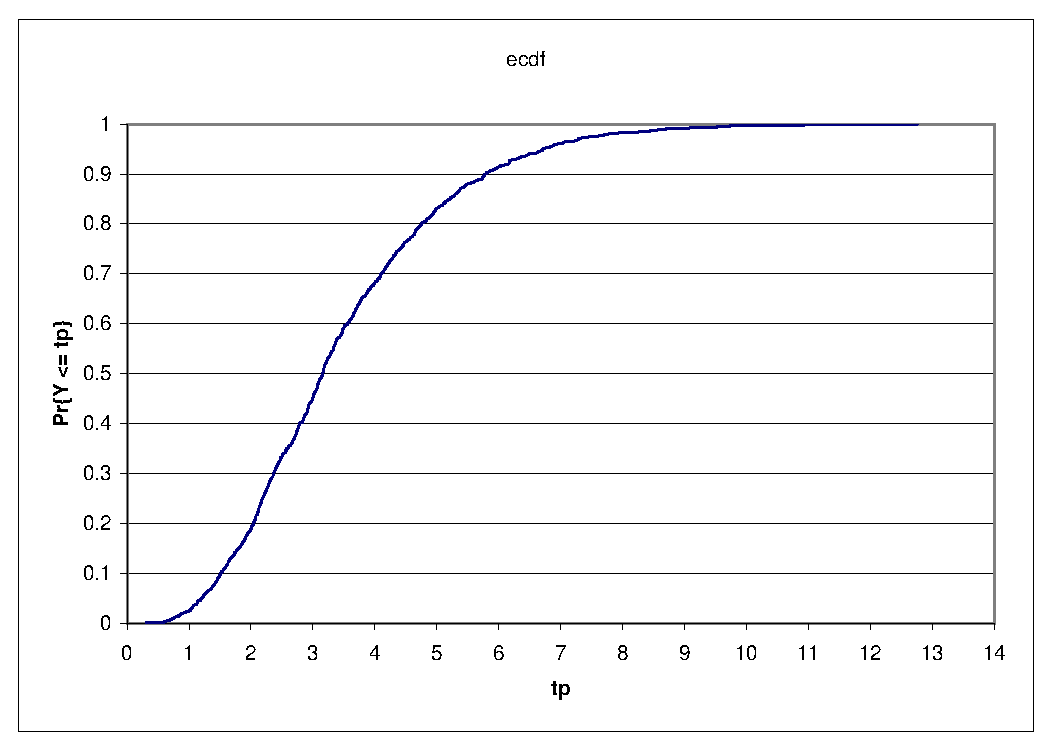
\includegraphics[width=4in]{SANecdf.eps}}
\caption{Empirical cdf of the project completion times.}
\label{fig:SANecdf}
\end{figure}

One other VBA feature that we use extensively in this example is the
ability to define constants, meaning variables whose values are fixed
once and for all in the simulation. This is done to make the
simulation more readable. For instance,
\begin{verbatim}
Const a As Integer = 1, b As Integer = 2,_
      c As Integer = 3, d As Integer = 4
Const InTo As Integer = 1, OutOf As Integer = 2
\end{verbatim}
By doing this we avoid the need to remember that node $c$ corresponds
to the number $3$, and what index corresponds to incoming vs.\
outgoing activities to a node.


Notice (see Fig.~\ref{fig:san.de.main}) that the simulation ends
when there are no additional activities remaining to be completed.
This can be checked via \texttt{Calendar.N}, a method that provides
the number of events currently on the event calendar.  

A difference
between this implementation of the SAN simulation and the one in
Sect.~\ref{sec:san.max.sim} is that here we write out the actual
time the project completes on each replication. By doing so, we can
estimate $\Pr\{Y > t_p\}$ for any value of $t_p$ by sorting the data
and counting how many out of $1000$ replications were greater than
$t_p$. Figure~\ref{fig:SANecdf} shows the empirical cdf of the $1000$
project completion times, which is the simulation estimate
of Eq.~(\ref{eq:san.analytic}).



\subsection{Issues and Extensions}
\label{sec:sim.san.issues}

\begin{enumerate}

\item In real projects there are not only activities, but also
limited and often shared resources that are needed to complete the
activities. Further, there may be specific resource allocation rules
when multiple activities contend for the same resource. How might
this be modeled in VBASim?

\item Time to complete the project is an important overall measure,
but at the planning stage it may be more important to discover which
activities or resources are the most critical to on-time completion
of the project. What additional output measures might be useful for
deciding which activites are ``critical?''

\end{enumerate}


\section{Simulating the Asian Option}
\label{sec:sim.asian}
\index{Asian option}


Here we consider estimating the value of an Asian option
\[
\nu = \E\left[ \mathrm{e}^{-rT} (\bar{X}(T) - K)^+ \right] 
\]
as described in Sect.~\ref{sec:fe}, where the maturity is $T = 1$
year, the risk-free interest rate is $r = 0.05$ and the strike price
is $K = \$55$. The underlying asset has an initial value of $X(0) =
\$50$ and the volitility is $\sigma^2 = (0.3)^2$.  Recall that the
key quantity is
\[
\bar{X}(T) = \frac{1}{T}\int_0^T X(t)\, \D t 
\]
the time average of a continuous-time, continuous-state geometric
Brownian motion 
process which we cannot truely simulate on a digital computer.
\index{geometric Brownian motion}
Thus, we approximate it by dividing the
interval $[0, T]$ into $m$ steps of size $\Delta t =
T/m$ and using the discrete approximation
\[
\widehat{\bar{X}(T)} = \frac{1}{m}
\sum_{i=1}^m X(i \Delta t) .
\]
This makes simulation possible, since 
\[
X(t_{i+1}) = X(t_i) \exp\left\{\left( r - \frac{1}{2}\sigma^2
\right)(t_{i+1}
- t_i) + \sigma\sqrt{t_{i+1} - t_i} \, Z_{i+1} \right\}
\]
for any increasing sequence of times $\{t_0, t_1, \ldots, t_m\}$, 
where $Z_1, Z_2, \ldots, Z_m$ are i.i.d.\ $\mathrm{N}(0,1)$. 

Figure~\ref{fig:asian.sim} is VBASim code that uses $m=32$ steps in
the approximation, and makes $10{,}000$ replications to estimate
$\nu$. Discrete-event structure would slow execution without any
obvious benefit, so a simple loop is used to advance time. The value
of the option from each replication is written to Excel for
post-simulation analysis.

The estimated value of $\nu$ is \$2.20 with a relative error of just over 2\%
(recall that the relative error is the standard error divided by the
mean). As the histogram in Fig.~\ref{fig:AsianHistogram} shows, the
option is frequently worthless (approximately 68\% of the time), but
the average payoff, conditional on the payoff being positive, is
approximately \$6.95.


\begin{figure}[tb]
\begin{center}
\begin{minipage}[t]{6in}\small
\begin{verbatim}
Private Sub AsianOption()
' Simulation of an Asian Option

Dim Replications As Integer
Dim Maturity As Double, Steps As Double
Dim i As Integer, j As Integer
Dim X As Double, Z As Double, InitialValue As Double
Dim Sigma As Double, Sigma2 As Double
Dim Sum As Double, Value As Double
Dim Interval As Double
Dim InterestRate As Double, StrikePrice As Double

' Set option parameters
Replications = 10000
Maturity = 1
Steps = 32
Sigma = 0.3
InterestRate = 0.05
InitialValue = 50
StrikePrice = 55
Interval = Maturity / Steps
Sigma2 = Sigma * Sigma / 2

Call Report("Option Value", "Option", 1, 1)
Call InitializeRNSeed
For i = 1 To Replications
    Sum = 0
    X = InitialValue
    For j = 1 To Steps
        Z = Normal(0, 1, 12)
        X = X * VBA.Exp((InterestRate - Sigma2) * Interval +  _
                Sigma * VBA.Sqr(Interval) * Z)
        Sum = Sum + X
    Next j
    Value = VBA.Exp(-InterestRate * Maturity) * _
                WorksheetFunction.Max(Sum / Steps - StrikePrice, 0)
    Call Report(Value, "Option", i + 1, 1)
Next i

End
End Sub
\end{verbatim}
\end{minipage}
\end{center}
\caption{VBA Simulation of the Asian option problem.}
\label{fig:asian.sim}
\end{figure}


\begin{figure}[tb]
\centerline{\includegraphics[width=4in]{AsianHistogram.eps}}
\caption{Histogram of the realized value of the Asian option from
10{,}000 replications.}
\label{fig:AsianHistogram}
\end{figure}

\section{Case Study: Service Center Simulation}
\label{sec:fax}

This section presents a simulation case based on a project provided by
a former student. While still relatively simple, it is more complex
than the previous stylized examples, and the answer is not known
without simulating. The purpose of this section is to illustrate how
one might attack simulation modeling and programming for a realistic
problem.

\begin{example}[Fax Center Staffing] \label{ex:fax}

A service center receives faxed orders throughout the day,
with the rate of arrival varying hour by hour. The arrivals are
modeled by a nonstationary Possion process with the rates
shown in Table~\ref{tab:fax.arrivals}. \index{nonstationary Poisson
process}

\begin{table}[tb]
\caption{Arrival rate of faxes by hour.}
\label{tab:fax.arrivals}
\begin{center}
\begin{tabular}{lc}\hline
\multicolumn{1}{c}{Time}&Rate (faxes/minute) \\\hline
8 AM--9 AM & 4.37 \\
9 AM--10 AM & 6.24 \\
10 AM--11 AM & 5.29 \\
11 AM--12 PM & 2.97 \\
12 PM--1 PM & 2.03 \\
1 PM--2 PM & 2.79 \\
2 PM--3 PM & 2.36 \\
3 PM--4 PM & 1.04 \\\hline
\end{tabular}
\end{center}
\end{table}


A team of Entry Agents select faxes on a first-come-first-served basis
from the fax queue. Their time to process a fax is modeled as normally
distributed with mean $2.5$ minutes and standard deviation $1$ minute.
There are two possible outcomes after the Entry Agent finishes
processing a fax: either it was a simple fax and the work on it is
complete, or it was not simple and it needs to go to a Specialist for
further processing.  Over the course of a day, approximately 20\% of
the faxes require a Specialist.  The time for a Specialist to process
a fax is modeled as normally distributed with mean $4.0$ minutes and
standard deviation $1$ minute.  

Minimizing the number of staff minimizes cost, but certain
service-level requirements much be achieved.  In particular, 96\% of
all simple faxes should be completed within $10$ minutes of their
arrival, while 80\% of faxes requiring a Specialist should also be
completed (by both the Entry Agent and the Specialist) within $10$
minutes of their arrival.  

The service center is open from 8 AM to 4 PM daily, and it is possible
to change the staffing level at 12 PM. Thus, a staffing policy
consists of four numbers: the number of Entry Agents and Specialists
before noon, and the number of Entry Agents and Specialists after
noon.  Any fax that starts its processing before noon completes
processing by that same agent before the agent goes off duty; and
faxes in the queues at the end of the day are processed before the
agents leave work and therefore are not carried over to the next day.

\end{example}

\emph{The first step in building any simulation model is deciding
what question or questions that the model should answer.} Knowing the
questions helps identify the system performance measures that the
simulation needs to estimate, which in turn drives the scope and level
of detail in the simulation model.

The grand question for the service center is, what is the minimum
number of Entry Agents and Specialists needed for both time
periods to meet the service-level requirements?  Therefore, the
simulation must at least provide an estimate of the percentage of
faxes of each type entered within 10 minutes, given a specific staff
assignment.

Even when there seems to be a clear overall objective (minimize the
staff required to achieve the service-level requirement), we often
want to consider trade offs around that objective. For instance, if
meeting the requirement requires a staff that is so large that they
are frequently underutilized, or if employing the minimal staff means
that the Entry Agents or Specialists frequently have to work well past
the end of the day, then we might be willing to alter the
service requirement a bit.  Statistics on the number and the time
spent by faxes in queue, and when the last fax of each day is actually
completed, provide this information. Including additional measures
of system performance, beyond the most critical ones, makes the
simulation more useful.

Many discrete-event, stochastic simulations involve entities that
dynamically flow through some sort of queueing network where they
compete for resources. In such simulations, identifying the entities
and resources is a good place to start the model. For this service
center the faxes are clearly the dynamic entities, while the Entry
Agents and Specialists are resources. The fax machines themselves
might also be considered a resource, especially if they are heavily
utilized or if outgoing as well as incoming faxes use the same
machines. It turns out that for this service center there is a bank of
fax machines dedicated to incoming faxes, so it is reasonable to treat
the arrival of faxes as an unconstrained external arrival process.
This fact was not stated in the original description of the problem;
follow-up questions are often needed to fully understand the system of
interest.

Whenever there are scarce resources, queues may form. Queues are often
first-in-first-out, with one queue for each resource, as they are in
this service center. However, queues may have priorities,
and multiple queues may be served by the same resource, or a single
queue may feed multiple resources. Queueing behavior is often a
critical part of the model. 

When the simulation involves entities flowing through a network of
queues, then there can be two types of arrivals: arrivals from outside
of the network and arrivals internal to the network. Outside
arrivals are like those we have already seen in the $M(t)/M/\infty$ and
$M/G/1$ examples.  Internal arrivals are departures from one queue
that become arrivals to others. How these are modeled depends largely
on whether the departure from one queue is an immediate arrival to the
next---in which case the departure and arrival events are effectively
the same thing---or whether there is some sort of transportation
delay---in which case the arrival to the next queue should be
scheduled as a distinct event.
For the service center the arrival of faxes to the Entry
Agents is an outside arrival process, while the 20\% of faxes that
require a Specialist are internal arrivals from the Entry Agents to
the Specialists. 

Critical to experiment design is defining what constitutes a
replication. Replications should be independent and identically
distributed. Since the service center does not carry faxes over from
one day to the next, a ``day'' defines a replication. If faxes did
carry over, but all faxes are cleared weekly, then a replication might
be defined by a work week. However, if there is always significant
carry over from one day to the next, then a replication might have to
be defined arbitrarily.

The work day at the service center is eight hours;
however the staff does not leave until all faxes that arrive before 4
PM are processed. If we defined a replication to be exactly eight
hours then we could be fooled by a staffing policy that allows a large
queue of faxes to build up toward the end of the day, since the entry
of those faxes would not be included in our statistics. To model a
replication that ends when there is no additional work remaining, we
will cut off the fax arrivals at 4 PM and then end the simulation when
the event calendar is empty. This works because idle Entry Agents and
Specialists will always take a fax from their queue if one is
available.

Rather than walk through the VBASim code line by line, we will point
out some highlights to facilitate the reader's understanding of the
code.

Figure~\ref{fig:fax.global} shows the global declarations for the
service center simulation. Of particular note are the two \DTStat\
statements defining \texttt{Regular10} and \texttt{Special10}. These
will be used to obtain the fraction of regular and special faxes that
are processed within the $10$-minute requirement by recording a $1$
for any fax that meets the requirement, and a $0$ otherwise. The mean
of these values is the desired fraction.


\begin{figure}[tbp]\small
\begin{verbatim}
' FaxCenter Simulation
' Parameters we may want to change
Dim MeanRegular As Double       ' mean entry time regular faxes
Dim VarRegular As Double        ' variance entry time regular faxes
Dim MeanSpecial As Double       ' mean entry time special faxes
Dim VarSpecial As Double        ' variance entry time special faxes
Dim RunLength As Double         ' length of the working day
Dim NumAgents As Integer        ' number of regular agents
Dim NumSpecialists As Integer   ' number of special agents
Dim NumAgentsPM As Integer      ' number of regular agents after noon
Dim NumSpecialistsPM As Integer ' number of special agents after noon

' Global objects needed for simulation
Dim RegularQ As New FIFOQueue       ' queue for all faxes
Dim SpecialQ As New FIFOQueue       ' queue for special faxes
Dim RegularWait As New DTStat       ' discrete-time statistics on fax waiting
Dim SpecialWait As New DTStat       ' discrete-time statistics on special fax waiting
Dim Regular10 As New DTStat         ' discrete-time statistics on < 10 minutes threshold
Dim Special10 As New DTStat         ' discrete-time statistics on < 10 minutes threshold
Dim Agents As New Resource          ' entry agents resource
Dim Specialists As New Resource     ' specialists resource
Dim ARate(1 To 8) As Double         ' arrival rates
Dim MaxRate As Double               ' maximum arrival rate
Dim Period As Double                ' period for which arrival rate stays constant
Dim NPeriods As Integer             ' number of periods in a "day"
\end{verbatim}
\caption{Global declarations for service center simulation.}
\label{fig:fax.global}
\end{figure}

\clearpage

The main program for the simulation is in Fig.~\ref{fig:fax.main}.
Of particular importance is the condition that ends the main simulation
loop: 
\begin{center}
\texttt{Loop Until Calendar.N = 0}
\end{center} 
The \texttt{N} method of
\Calendar\ returns the current number of pending events.  When the
event calendar is empty, then there are no additional faxes to
process, and no pending arrival of a fax. This condition will only
hold after 4 PM and once all remaining faxes have been entered.

Also notice the event \texttt{ChangeStaff}, which is scheduled to
occur at noon ($240$ minutes). Here we use the \texttt{SetUnits}
method of the \Resource\ to change the staffing levels. The reader
should look at the VBASim \Resource\ class object and convince
themselves that even if we reduce the number of staff at noon the
faxes in process will not be affected.

The staffing policy to be simulated is read in from four cells of the worksheet
\texttt{Fax}. By placing a VBA control button to start the simulation on
the worksheet we can simulate different staffing policies, and view
the results, without actually touching the VBA code.

The function \verb+NSPP_Fax+ generates the interarrival times for
faxes with the desired time-varying rate; this function will be
described in Chap.~\ref{ch:input}.

\begin{figure}[tbp]\small
\begin{verbatim}
Public Sub FaxCenterSim()
    Dim Reps As Integer
    Dim NextEvent As EventNotice  
' Read in staffing policy
    NumAgents = Worksheets("Fax").Cells(25, 5)
    NumAgentsPM = Worksheets("Fax").Cells(25, 6)
    NumSpecialists = Worksheets("Fax").Cells(26, 5)
    NumSpecialistsPM = Worksheets("Fax").Cells(26, 6)
    Call MyInit
    For Reps = 1 To 10
        Call VBASimInit
        Agents.SetUnits (NumAgents)
        Specialists.SetUnits (NumSpecialists)
        Call Schedule("Arrival", NSPP_Fax(ARate, MaxRate, NPeriods, Period, 1))
        Call Schedule("ChangeStaff", 4 * 60)   
        Do
            Set NextEvent = Calendar.Remove
            Clock = NextEvent.EventTime
            Select Case NextEvent.EventType
            Case "Arrival"
                Call Arrival
            Case "EndOfEntry"
                Call EndOfEntry(NextEvent.WhichObject)
            Case "EndOfEntrySpecial"
                Call EndOfEntrySpecial(NextEvent.WhichObject)
            Case "ChangeStaff"
                Agents.SetUnits (NumAgentsPM)
                Specialists.SetUnits (NumSpecialistsPM)
            End Select
        Loop Until Calendar.N = 0 ' stop when event calendar empty
' Write output report for each replication
        Call Report(RegularWait.Mean, "Fax", Reps + 1, 1)
        Call Report(RegularQ.Mean, "Fax", Reps + 1, 2)
        Call Report(Agents.Mean, "Fax", Reps + 1, 3)
        Call Report(SpecialWait.Mean, "Fax", Reps + 1, 4)
        Call Report(SpecialQ.Mean, "Fax", Reps + 1, 5)
        Call Report(Specialists.Mean, "Fax", Reps + 1, 6)
        Call Report(Regular10.Mean, "Fax", Reps + 1, 7)
        Call Report(Special10.Mean, "Fax", Reps + 1, 8)
        Call Report(Clock, "Fax", Reps + 1, 9)
    Next Reps
    End
End Sub
\end{verbatim}
\caption{Main program for service center simulation.}
\label{fig:fax.main}
\end{figure}

\clearpage

Figure~\ref{fig:fax.entry} contains the arrival and end-of-entry
events for faxes at the Entry Agents. The next arrival is scheduled
only if \texttt{Clock < RunLength}; in this way we cut off fax
arrivals after 4 PM. The \texttt{EndOfEntry} event passes 20\% of the
faxes directly and immediately to the Specialists by executing
\texttt{Call SpecialArrival(DepartingFax)} and passing the pointer to
the \texttt{DepartingFax} entity. Equivalently, we could have
scheduled a \texttt{SpecialArrival} event to occur zero time units
into the future (or nonzero time units if it takes time to transport
the fax).

The \texttt{Record} method of the \DTStat\ \texttt{Regular10} is used to
collect a $0$ or $1$ depending on whether the total wait was less than
10 minutes.

The arrival and end-of-entry events for the
Specialists, shown in Fig.~\ref{fig:fax.specialists}, work similarly
to those of the Entry Agents.

Initializations that occur once are shown in Fig.~\ref{fig:fax.initial}.

Ten replications of this simulation with a staffing policy of $15$
Entry Agents in the morning and $9$ in the afternoon, and $6$
Specialists in the morning and $3$ in the afternoon, gives $0.98 \pm
0.02$ for the fraction of regular faxes entered in $10$ minutes or
less, and $0.81 \pm 0.06$ for the special faxes. The ``$\pm$'' are
$95$\% confidence intervals. This policy appears to be close to the
requirements, although if we absolutely insist on $80$\% for the
special faxes then additional replications are needed to narrow the
confidence interval.


\begin{figure}[tbp]\small
\begin{verbatim}
Private Sub Arrival()
' Schedule next fax arrival if < 4 PM
    If Clock < RunLength Then
        Call Schedule("Arrival", NSPP_Fax(ARate, MaxRate, NPeriods, Period, 1))
    Else
        Exit Sub
    End If
' Process the newly arriving Fax
    Dim Fax As New Entity
    If Agents.Busy < Agents.NumberOfUnits Then
        Agents.Seize (1)
        Call SchedulePlus("EndOfEntry", Normal(MeanRegular, VarRegular, 2), Fax)
    Else
        RegularQ.Add Fax
    End If
    Set Fax = Nothing
End Sub

Private Sub EndOfEntry(DepartingFax As Entity)
    Dim Wait As Double
' Record wait time if regular; move on if special
    If Uniform(0, 1, 3) < 0.2 Then
        Call SpecialArrival(DepartingFax)
    Else
        Wait = Clock - DepartingFax.CreateTime
        RegularWait.Record (Wait)
        If Wait < 10 Then
            Regular10.Record (1)
        Else
            Regular10.Record (0)
        End If
    End If
    Set DepartingFax = Nothing
' Check to see if there is another Fax; if yes start entry
' otherwise free the agent
    If RegularQ.NumQueue > 0 And Agents.NumberOfUnits >= Agents.Busy Then
        Set DepartingFax = RegularQ.Remove
        Call SchedulePlus("EndOfEntry", Normal(MeanRegular,_
           VarRegular, 2), DepartingFax)
        Set DepartingFax = Nothing
    Else
        Agents.Free (1)
    End If   
End Sub
\end{verbatim}
\caption{Events for Entry Agents.}
\label{fig:fax.entry}
\end{figure}


\begin{figure}[tbp]\small
\begin{verbatim}
Private Sub SpecialArrival(SpecialFax As Entity)
' If special agent available, start entry by seizing the special agent
    If Specialists.Busy < Specialists.NumberOfUnits Then
        Specialists.Seize (1)
        Call SchedulePlus("EndOfEntrySpecial", Normal(MeanSpecial, _ 
           VarSpecial, 4), SpecialFax)
    Else
        SpecialQ.Add SpecialFax
    End If
    Set SpecialFax = Nothing  
End Sub

Private Sub EndOfEntrySpecial(DepartingFax As Entity)
    Dim Wait As Double
' Record wait time and indicator if < 10 minutes
    Wait = Clock - DepartingFax.CreateTime
    SpecialWait.Record (Wait)
    If Wait < 10 Then
        Special10.Record (1)
    Else
        Special10.Record (0)
    End If
    Set DepartingFax = Nothing
' Check to see if there is another Fax; if yes start entry
' otherwise free the specialist
    If SpecialQ.NumQueue > 0 And Specialists.NumberOfUnits >= Specialists.Busy Then
        Set DepartingFax = SpecialQ.Remove
        Call SchedulePlus("EndOfEntrySpecial", Normal(MeanSpecial, _
           VarSpecial, 4), DepartingFax)
        Set DepartingFax = Nothing
    Else
        Specialists.Free (1)
    End If  
End Sub
\end{verbatim}
\caption{Events for Specialists.}
\label{fig:fax.specialists}
\end{figure}

\clearpage 


\begin{figure}[tbp]
\begin{verbatim}
Private Sub MyInit()
    Call InitializeRNSeed
    MeanRegular = 2.5
    VarRegular = 1#
    MeanSpecial = 4
    VarSpecial = 1#
    RunLength = 480
' Add queues, resources and statistics that need to be
' initialized between replications to the global collections
    TheDTStats.Add RegularWait
    TheDTStats.Add SpecialWait
    TheDTStats.Add Regular10
    TheDTStats.Add Special10
    TheQueues.Add RegularQ
    TheQueues.Add SpecialQ
    TheResources.Add Agents
    TheResources.Add Specialists
' Write headings for the output reports
    Call Report("Ave Reg Wait", "Fax", 1, 1)
    Call Report("Ave Num Reg Q", "Fax", 1, 2)
    Call Report("Agents Busy", "Fax", 1, 3)
    Call Report("Ave Spec Wait", "Fax", 1, 4)
    Call Report("Ave Num Spec Q", "Fax", 1, 5)
    Call Report("Specialists Busy", "Fax", 1, 6)
    Call Report("Reg < 10", "Fax", 1, 7)
    Call Report("Spec < 10", "Fax", 1, 8)
    Call Report("End Time", "Fax", 1, 9)
' Arrival process data
    NPeriods = 8
    Period = 60
    MaxRate = 6.24
    ARate(1) = 4.37
    ARate(2) = 6.24
    ARate(3) = 5.29
    ARate(4) = 2.97
    ARate(5) = 2.03
    ARate(6) = 2.79
    ARate(7) = 2.36
    ARate(8) = 1.04
End Sub
\end{verbatim}
\caption{Initializations for service center simulation.}
\label{fig:fax.initial}
\end{figure}

\subsection{Issues and Extensions}
\label{sec:sim.fax.issues}

\begin{enumerate}

\item There are many similarities between the programming for this
simulation and the event-based simulation of the $M/G/1$ queue.
However, there is an important difference that is due to having
muliple agents. For the $M/G/1$ queue, a single \FIFOQueue\ object
held both the customer in service (who is at the front of the queue)
and the customers waiting for service. This approach does not work for
the Fax Center because when there are multiple agents the faxes need
not complete entry in the same order in which they arrive. To
accomodate this, the \FIFOQueue\ holds only those faxes waiting for
entry, and the \Entity\ representing a fax that is being entered is
stored with the \EventNotice\ for the end-of-entry event. This is
accomplished by the statement 
\begin{center}
\begin{verbatim}
Call SchedulePlus("EndOfEntry", _ 
   Normal(MeanRegular, VarRegular, 2), DepartingFax)
\end{verbatim}
\end{center}
\texttt{SchedulePlus} allows an object (\texttt{DepartingFax} in this
case) to be assigned to the
\texttt{.WhichObject} property of the \EventNotice.
The \Entity\ can then be passed to the event using the statement
\begin{center}
\texttt{Call EndOfEntry(NextEvent.WhichObject)}
\end{center}


\item The fax entry times were modeled as being normally distributed.
However, the normal distribution admits negative values, which
certainly does not make sense. What should be done about this?
Consider mapping negative values to 0, or generating a new value
whenever a negative value occurs. Which is more likely to be realistic
and why?

\end{enumerate}

\section*{Exercises}
\addcontentsline{toc}{section}{Exercises}

\begin{enumerate}

\item For the hospital problem, simulate the current system in which the
receptionist's service time is well modeled as having an Erlang-$4$
distribution with mean $0.6$ minutes. Compare the waiting time to the
proposed electronic kiosk alternative. 

\item Simulate an $M(t)/G/\infty$ queue where $G$ corresponds to an
Erlang distribution with fixed mean but try different numbers of
phases. That is, keep the mean service time fixed but change the
variability. Is the expected number if queue sensitive to the
variance in the service time?

\item Modify the SAN simulation to allow each activity to have a
different mean time to complete (currently they all have mean time
$1$). Use a Collection to hold these mean times.

\item Try the following numbers of steps for approximating the value
of the Asian option to see how sensitive the value is to the step
size: $m=8, 16, 32, 64, 128$.

\item In the simulation of the Asian option, the sample mean of
10{,}000 replications was $2.198270479$, and the standard deviation
was $4.770393202$. Approximately how many replications would it take
to decrease the relative error to less than 1\%?

\item For the service center, increase the number of replications
until you can be confident that that suggested policy does or does not
achieve the $80$\% entry in less than $10$ minutes requirement for
special faxes.

\item For the service center, find the minimum staffing policy (in
terms of total number of staff) that achieves the service-level
requirement.  Examine the other statistics generated by the simulation
to make sure you are satisfied with this policy. 

\item For the service center, suppose that Specialists earn twice as
much as Entry Agents.  Find the minimum cost staffing policy that
achieves the service-level requirement. Examine the other statistics
generated by the simulation to make sure you are satisfied with this
policy. 

\item For the service center, suppose that the staffing level can
change hourly, but once an Agent or Specialist comes on duty they
must work for four hours. Find the minimum staffing policy (in
terms of total number of staff) that achieves the service-level
requirement.

\item For the service center, pick a staffing policy that fails to
achieve the service level requirements by $20$\% or more. Rerun the
simulation with a replication being defined as exactly 8 hours, but do
not carry waiting faxes over to the next day. How much do the
statistics differ using the two different ways to end a replication?


\item The function \verb+NSPP_Fax+ is listed below. This function
implements the thinning method described in
Sect.~\ref{sec:sim.mminf} for a nonstationary Poisson process with
piecewise-constant rate function. Study it and describe how it works.
\index{nonstationary Poisson process} \index{thinning}

\small
\begin{verbatim}
Private Function NSPP_Fax(ARate() As Double, MaxRate As Double, NPeriods As Integer, _
                Period As Double, Stream As Integer) As Double
' This function generates interarrival times from a NSPP with piecewise constant
' arrival rate over a fixed time of Period*NPeriod time units

' ARate = array of arrival rates over a common length Period
' MaxRate = maximum value of ARate
' Period = time units between (possible) changes in arrival rate
' NPeriods = number of time periods in ARate
Dim i As Integer
Dim PossibleArrival As Double
PossibleArrival = Clock + Expon(1 / MaxRate, Stream)
i = WorksheetFunction.Min(NPeriods, _
    WorksheetFunction.Ceiling(PossibleArrival / Period, 1))
Do Until Uniform(0, 1, Stream) < ARate(i) / MaxRate
    PossibleArrival = PossibleArrival + Expon(1 / MaxRate, Stream)
    i = WorksheetFunction.Min(NPeriods, _
    WorksheetFunction.Ceiling(PossibleArrival / Period, 1))
Loop
NSPP_Fax = PossibleArrival - Clock            
End Function
\end{verbatim} \normalsize


\item  Beginning with the event-based $M/G/1$ simulation,
implement the changes necessary to make it an $M/G/s$ simulation (a
single queue with any number of servers). Keeping $\lambda = 1$ and
$\tau/s = 0.8$, simulate $s=1,2,3$ servers and compare the results.
What you are doing is comparing queues with the same service capacity,
but with $1$ fast server as compared to two or more slower servers.
State clearly what you observe.

\item  Modify the VBASim event-based simulation of the $M/G/1$
queue to simulate an M/G/1/$c$ retrial queue. This means that customers
who arrive to find $c$ customers in the system (including the customer
in service) leave immediately, but arrive again after an exponentially
distributed amount of time with mean \texttt{MeanTR}.  Hint: The
existence of retrial customers should not affect the arrival process for
first-time arrivals. 

\item  This problem assumes a more advanced background in
stochastic processes. In the simulation of the $M(t)/M/\infty$ queue
there could be a very large number of events on the event calendar: one
``Arrival'' and one ``Departure'' for \textit{each} car currently in the
garage. However, properties of the exponential distribution can reduce
this to no more than two events.  Let $\beta = 1/\tau$ be the departure
rate for a car (recall that $\tau$ is the mean parking time). If at any
time we observe that there are $N$ car in the garage (no matter how long
they have been there), then the time until the first of these cars
departs is exponentially distributed with mean $1/(N\beta)$. Use this
insight to build an $M(t)/M/\infty$ simulation with at most two pending
events, next arrival and next departure. Hint: Whenever an arrival
occurs the distribution of the time until the next departure changes, so
the scheduled next departure time must again be generated.


\item  The phone desk for a small office is staffed from 8 AM
to 4 PM by a single operator. Calls arrive according to a Poisson
process with rate 6 per hour, and the time to serve a call is uniformly
distributed between 5 and 12 minutes.  Callers who find the operator
busy are placed on hold, if there is space available, otherwise they
receive a busy signal and the call is considered ``lost.'' In addition,
10\% of callers who do not immediately get the operator decide to hang
up rather than go on hold; they are not considered lost, since it was
their choice. Because the hold queue occupies resources, the company
would like to know the smallest capacity (number of callers) for the
hold queue that keeps the daily fraction of lost calls under 5\%. In
addition, they would like to know the long-run utilization of the
operator to make sure he or she will not be too busy.  Use VBASim to
simulate this system and find the required capacity for the hold queue.
Model the callers as class \texttt{Entity}, the hold queue as class
\texttt{FIFOQueue} and the operator as class \texttt{Resource}.  Use the
VBASim functions \texttt{Expon} and \texttt{Uniform} for random-variate
generation.  Use class \texttt{DTStat} to estimate the fraction of calls
lost (record a 0 for calls not lost, a 1 for those that are lost so that
the sample mean is the fraction lost). Use the statistics collected by class
\texttt{Resource} to estimate the utilization. 


\item \label{ex:smp} Software Made Personal (SMP)
customizes software products in two areas: financial tracking and
contact management.  They currently have a customer support call
center that handles technical questions for owners of their software
from the hours of 8 AM to 4 PM Eastern Time.

When a customer calls they the first listen to a recording that asks
them to select among the product lines; historically 59\% are financial
products and 41\% contact management products. The number of customers
who can be connected (talking to an agent or on hold) at any one time is
essentially unlimited.  Each product line has its own agents. If an
appropriate agent is available then the call is immediately routed to
the agent; if an appropriate agent is not available, then the caller is
placed in a hold queue (and listens to a combination of music and ads).
SMP has observed that hang ups very rarely happen.

SMP is hoping to reduce the total number of agents they need by
cross-training agents so that they can answer calls for any product
line.  Since the agents will not be experts across all products, this
is expected to increase the time to process a call by about 5\%.  The
question that SMP has asked you to answer is how many cross-trained
agents are needed to provide service at the same level as the current
system.

Incoming calls can be modeled as a Poisson arrival process with a rate
of $60$ per hour.  The mean time required for an agent to answer a
question is $5$ minutes, with the actual time being Erlang-$2$ for
financial calls, and Erlang-$3$ for contact management calls.  The
current assignment of agents is $4$ for financial and $3$ for contact
management.  Simulate the system to find out how many agents are
needed to deliver the same level of service in the cross-trained system
as in the current system. 


\end{enumerate}


\end{document}